% !TEX program = pdflatex
\documentclass{article}
% FONTS
\usepackage[T1]{fontenc}
\usepackage{tgtermes}
\usepackage{amsmath}

% GEOMETRY
\usepackage[
  paper  = letterpaper,
  left   = 1.65in,
  right  = 1.65in,
  top    = 1.0in,
  bottom = 1.0in,
  ]{geometry}

% COLOR
\usepackage[usenames,dvipsnames]{xcolor}
\definecolor{shadecolor}{gray}{0.9}

% SPACING and TEXT
\usepackage[final,expansion=alltext]{microtype}
\usepackage[english]{babel}
\usepackage[parfill]{parskip}
\usepackage{afterpage}
\usepackage{framed}
\usepackage{nicefrac}

% COUNTERS
\renewcommand{\labelenumi}{\color{black!67}{\arabic{enumi}.}}
\renewcommand{\labelenumii}{{\color{black!67}(\alph{enumii})}}
\renewcommand{\labelitemi}{{\color{black!67}\textbullet}}

% FIGURES
\usepackage{graphicx}
\usepackage[labelfont=bf]{caption}
\usepackage[format=hang]{subcaption}

% TABLES
\usepackage{booktabs}

% BIBLIOGRAPHY
\usepackage{natbib}

% ALGORITHMS
\usepackage[algoruled]{algorithm2e}
\usepackage{listings}
\usepackage{fancyvrb}
\fvset{fontsize=\normalsize}

% HYPERREF
\usepackage[colorlinks,linktoc=all]{hyperref}
\usepackage[all]{hypcap}
\hypersetup{citecolor=Violet}
\hypersetup{linkcolor=black}
\hypersetup{urlcolor=MidnightBlue}

% CLEVEREF must come after HYPERREF
\usepackage[nameinlink]{cleveref}

% COLOR DEFINITIONS
\newcommand{\red}[1]{\textcolor{BrickRed}{#1}}
\newcommand{\orange}[1]{\textcolor{BurntOrange}{#1}}
\newcommand{\green}[1]{\textcolor{OliveGreen}{#1}}
\newcommand{\blue}[1]{\textcolor{MidnightBlue}{#1}}
\newcommand{\gray}[1]{\textcolor{black!60}{#1}}

% LISTINGS
\usepackage{listings}


% !TEX root = template.tex

% \DeclareRobustCommand{\mb}[1]{\ensuremath{\boldsymbol{\mathbf{#1}}}}
\DeclareRobustCommand{\mb}[1]{\mathbold{#1}}

% \newcommand{\KL}[2]{\ensuremath{\textrm{KL}\PARENS{#1\;\|\;#2}}}
\DeclareRobustCommand{\KL}[2]{\ensuremath{\textrm{KL}\left(#1\;\|\;#2\right)}}

\DeclareMathOperator*{\argmax}{arg\,max}
\DeclareMathOperator*{\argmin}{arg\,min}

\renewcommand{\mid}{~\vert~}
\newcommand{\g}{\mid}
\newcommand{\prm}{~;~}

\newcommand{\mba}{\mb{a}}
\newcommand{\mbb}{\mb{b}}
\newcommand{\mbc}{\mb{c}}
\newcommand{\mbd}{\mb{d}}
\newcommand{\mbe}{\mb{e}}
\newcommand{\mbg}{\mb{g}}
\newcommand{\mbh}{\mb{h}}
\newcommand{\mbi}{\mb{i}}
\newcommand{\mbj}{\mb{j}}
\newcommand{\mbk}{\mb{k}}
\newcommand{\mbl}{\mb{l}}
\newcommand{\mbm}{\mb{m}}
\newcommand{\mbn}{\mb{n}}
\newcommand{\mbo}{\mb{o}}
\newcommand{\mbp}{\mb{p}}
\newcommand{\mbq}{\mb{q}}
\newcommand{\mbr}{\mb{r}}
\newcommand{\mbs}{\mb{s}}
\newcommand{\mbt}{\mb{t}}
\newcommand{\mbu}{\mb{u}}
\newcommand{\mbv}{\mb{v}}
\newcommand{\mbw}{\mb{w}}
\newcommand{\mbx}{\mb{x}}
\newcommand{\mby}{\mb{y}}
\newcommand{\mbz}{\mb{z}}

\newcommand{\mbA}{\mb{A}}
\newcommand{\mbB}{\mb{B}}
\newcommand{\mbC}{\mb{C}}
\newcommand{\mbD}{\mb{D}}
\newcommand{\mbE}{\mb{E}}
\newcommand{\mbF}{\mb{F}}
\newcommand{\mbG}{\mb{G}}
\newcommand{\mbH}{\mb{H}}
\newcommand{\mbI}{\mb{I}}
\newcommand{\mbJ}{\mb{J}}
\newcommand{\mbK}{\mb{K}}
\newcommand{\mbL}{\mb{L}}
\newcommand{\mbM}{\mb{M}}
\newcommand{\mbN}{\mb{N}}
\newcommand{\mbO}{\mb{O}}
\newcommand{\mbP}{\mb{P}}
\newcommand{\mbQ}{\mb{Q}}
\newcommand{\mbR}{\mb{R}}
\newcommand{\mbS}{\mb{S}}
\newcommand{\mbT}{\mb{T}}
\newcommand{\mbU}{\mb{U}}
\newcommand{\mbV}{\mb{V}}
\newcommand{\mbW}{\mb{W}}
\newcommand{\mbX}{\mb{X}}
\newcommand{\mbY}{\mb{Y}}
\newcommand{\mbZ}{\mb{Z}}

\newcommand{\mbalpha}{\mb{\alpha}}
\newcommand{\mbbeta}{\mb{\beta}}
\newcommand{\mbdelta}{\mb{\delta}}
\newcommand{\mbepsilon}{\mb{\epsilon}}
\newcommand{\mbchi}{\mb{\chi}}
\newcommand{\mbeta}{\mb{\eta}}
\newcommand{\mbgamma}{\mb{\gamma}}
\newcommand{\mbiota}{\mb{\iota}}
\newcommand{\mbkappa}{\mb{\kappa}}
\newcommand{\mblambda}{\mb{\lambda}}
\newcommand{\mbmu}{\mb{\mu}}
\newcommand{\mbnu}{\mb{\nu}}
\newcommand{\mbomega}{\mb{\omega}}
\newcommand{\mbphi}{\mb{\phi}}
\newcommand{\mbpi}{\mb{\pi}}
\newcommand{\mbpsi}{\mb{\psi}}
\newcommand{\mbrho}{\mb{\rho}}
\newcommand{\mbsigma}{\mb{\sigma}}
\newcommand{\mbtau}{\mb{\tau}}
\newcommand{\mbtheta}{\mb{\theta}}
\newcommand{\mbupsilon}{\mb{\upsilon}}
\newcommand{\mbvarepsilon}{\mb{\varepsilon}}
\newcommand{\mbvarphi}{\mb{\varphi}}
\newcommand{\mbvartheta}{\mb{\vartheta}}
\newcommand{\mbvarrho}{\mb{\varrho}}
\newcommand{\mbxi}{\mb{\xi}}
\newcommand{\mbzeta}{\mb{\zeta}}

\newcommand{\mbDelta}{\mb{\Delta}}
\newcommand{\mbGamma}{\mb{\Gamma}}
\newcommand{\mbLambda}{\mb{\Lambda}}
\newcommand{\mbOmega}{\mb{\Omega}}
\newcommand{\mbPhi}{\mb{\Phi}}
\newcommand{\mbPi}{\mb{\Pi}}
\newcommand{\mbPsi}{\mb{\Psi}}
\newcommand{\mbSigma}{\mb{\Sigma}}
\newcommand{\mbTheta}{\mb{\Theta}}
\newcommand{\mbUpsilon}{\mb{\Upsilon}}
\newcommand{\mbXi}{\mb{\Xi}}

\newcommand{\mbone}{\mbf{1}}
\newcommand{\mbzero}{\mbf{0}}


\newcommand{\dif}{\mathop{}\!\mathrm{d}}
\newcommand{\diag}{\textrm{diag}}
\newcommand{\supp}{\textrm{supp}}

\newcommand{\E}{\mathbb{E}}
\newcommand{\Var}{\mathbb{V}\textrm{ar}}
\newcommand{\bbH}{\mathbb{H}}

\newcommand{\bbN}{\mathbb{N}}
\newcommand{\bbZ}{\mathbb{Z}}
\newcommand{\bbR}{\mathbb{R}}
\newcommand{\bbS}{\mathbb{S}}

\newcommand{\cA}{\mathcal{A}}
\newcommand{\cB}{\mathcal{B}}
\newcommand{\cC}{\mathcal{C}}
\newcommand{\cD}{\mathcal{D}}
\newcommand{\cE}{\mathcal{E}}
\newcommand{\cF}{\mathcal{F}}
\newcommand{\cG}{\mathcal{G}}
\newcommand{\cH}{\mathcal{H}}
\newcommand{\cI}{\mathcal{I}}
\newcommand{\cJ}{\mathcal{J}}
\newcommand{\cK}{\mathcal{K}}
\newcommand{\cL}{\mathcal{L}}
\newcommand{\cM}{\mathcal{M}}
\newcommand{\cN}{\mathcal{N}}
\newcommand{\cO}{\mathcal{O}}
\newcommand{\cP}{\mathcal{P}}
\newcommand{\cQ}{\mathcal{Q}}
\newcommand{\cR}{\mathcal{R}}
\newcommand{\cS}{\mathcal{S}}
\newcommand{\cT}{\mathcal{T}}
\newcommand{\cU}{\mathcal{U}}
\newcommand{\cV}{\mathcal{V}}
\newcommand{\cW}{\mathcal{W}}
\newcommand{\cX}{\mathcal{X}}
\newcommand{\cY}{\mathcal{Y}}
\newcommand{\cZ}{\mathcal{Z}}

\newcommand{\Gam}{\textrm{Gam}}
\newcommand{\InvGam}{\textrm{InvGam}}

\usepackage{amsfonts} 
\begin{document}

\title{Effect of prescribed fire on the wildfire in California}
\date{\today}
\author{Shuonan Chen, sc4417}

\maketitle

\begin{abstract}
Wildfires in California cause many socioecological damages. While the impact is huge and getting larger in recent decades, not much is known about their impact and what factors might contribute the severity levels. 
% Current analysis on wildfire oftentimes assume that the consequences caused by wildfire is uniform across the regions. 
Here we take a modeling aproach based on Gaussian Process and explore if previously prescribed fire and hydrologic regions have impact on the severity of wildfire in California. We found that the prescribed fire has relatively small negative impact on the wildfire severity. We also found that some of the hydrologic regions have a large effect, especially the coastal area are more likely to be affected by severe wildfire. The model can be further extended to incorporate more explanatory variables which will help the climate scientists to study the best strategy to minimize the negative effect of wildfire. 
\end{abstract}



\section{Introduction}
%wildfires
California wildfire are mainly caused by events such as lightning strikes and human activities. Even though from the environmental perspective, wildfires promote the re-vegetation and hence are a part of natural process in the forests, they cause many socioecological damages. For instance, severe wildfires can destroy the habitats for animals and plants, disrupt the power and water supply and transportation, and also can worsen the air pollution \cite{moritz2014learning}. 
With the extreme heat and driness caused by the global warming in recent decades, the California's winter season is getting shorter. As a consequence, we have witnessed an increase in the severe wildfire incidents and the negative impact caused. 


%wildfires and other factors, e.g., px fires. 
While it is almost impossible to completely prevent the wildfire from happening, their level of impacts can vary, depending on the vegetation conditions, landscape, water contents in the soil, or previously burned history. One of the age-old practises to reduce the disruptive effects of wildfires is to induce the planned fire burns, namely ``prescribed burn''. Prescribed burns have been used for the forest management by getting rid of the small trees and reducing the fuel load for the wildfires, and thus the wildfire is easier to control. The effectiveness of reducing the severity of wildfires by regular prescribed burn have been drawing more attentions in recent years. 


Wildfire severity is hard to estimate, and even if we do, the challenge remains to understand the relationship between the wildfire and the other factors. 
The lack of understanding on what factors are associated with the fire severity not only prevents us from interrupting the serious damage caused, but also makes it difficult to gain insights on the other effects. For instance, an effort was made to estimate the Giant Sequoia mortality rate in the wildfire \cite{stephenson2021preliminary}, which concluded that between 7,500 to 10,600 large sequoias were killed in the 2020 Castle fire. However in this study, the authors made a simplified assumption that the mortality of Giant Sequoia is proportional to the reported severity of the wildfire. This is a reasonable assumption based on our current understanding and available resources. However it is possible that some parts of the grove are burned more servery if the landscape is tilted, or the soil water contents are significantly different from the other regions with the similar wildfire severity. More detailed understanding of what factors might be relevant to the wildfire will benefit for both the analysis and the future wildfire prevention. 



In this study we explore these impact on wildfire severity. Particularly, we investigate if the prescribed burn and different geographical regions have impact on the burn severity of wildfires. Through this work, we provide the possible modeling framework to understand what factors might contribute to the severe wildfire in California, and used this modeling framework to understand the effects of hydrologic region and the prescribed fire at the same region. This work can be extended to give a more systematic understanding by incorporating more explanatory variables such as topography of the region and vegetation conditions. This framework can also be used to provide insights into the analytical methods, including the assumptions made by \cite{stephenson2021preliminary}, and give a more accurate estimate of the mortality rate of Giant Sequoia. 


\section{Methods}
\subsection*{Data source}
In total three data sources are used in this study, as shown in Figure \ref{fig:data}. The first is the burned area by wildfire, obtained from Rapid Assessment of Vegetation Condition After Wildfire (RAVG) website. We filtered the data based on the year to keep the fire that is recorded between 2017 asnd 2022. 




\begin{figure*}[t!]
  \centering
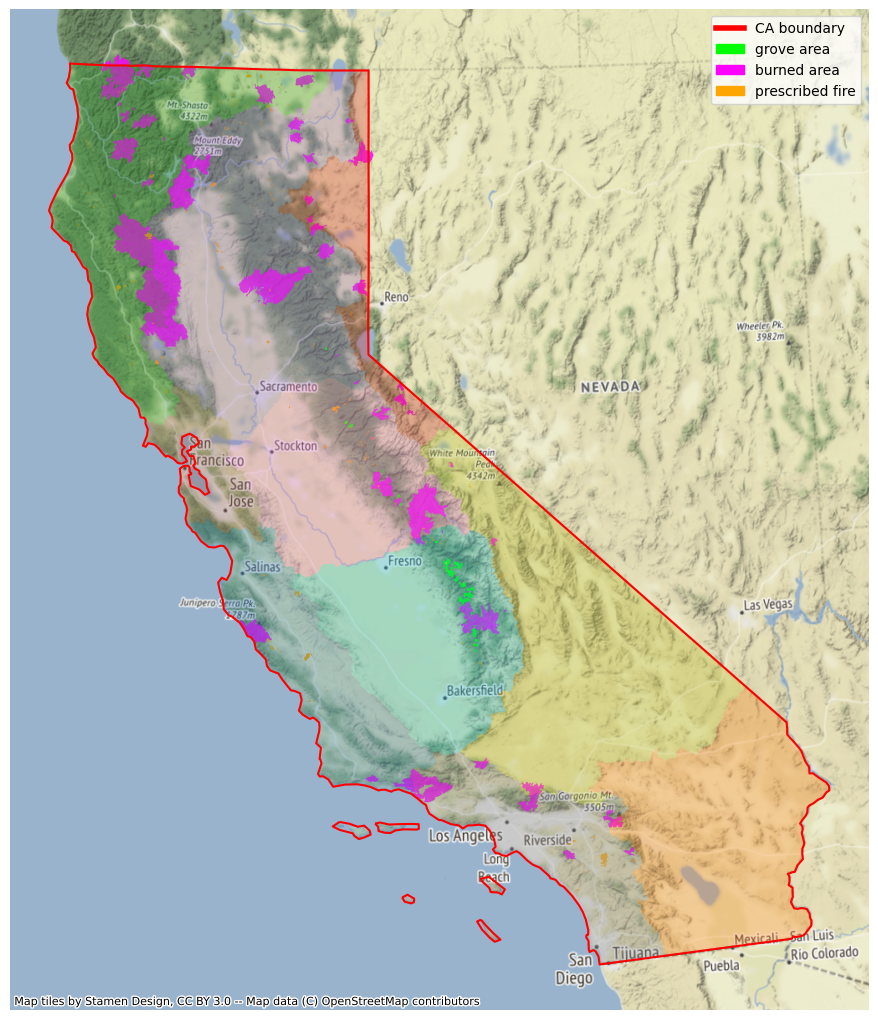
\includegraphics[width=0.49\textwidth]{latex_template/figs/prescribed_0.png}
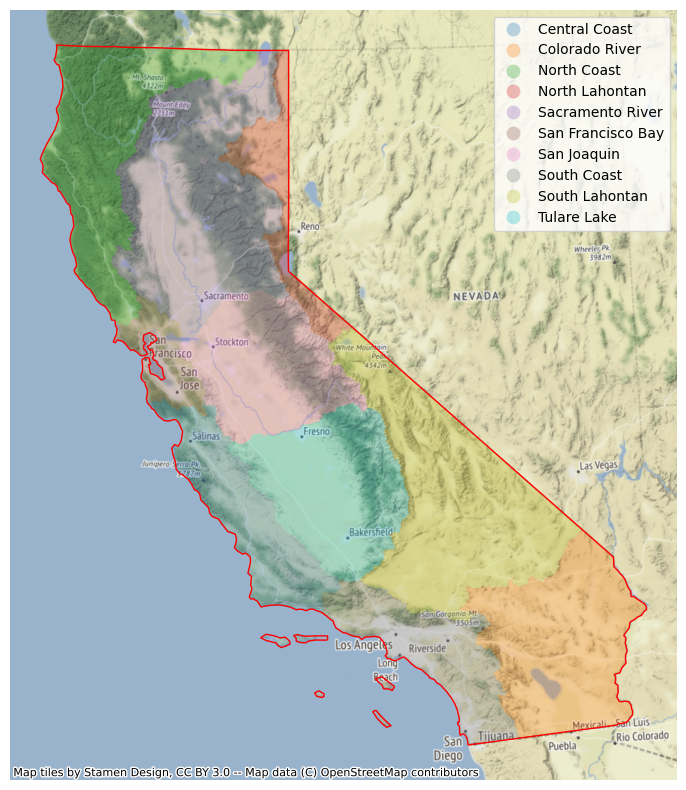
\includegraphics[width=0.49\textwidth]{figs/HRarea_1.png}
\caption{\textbf{Data description.} Left panel shows the prescribed fire (orange) location and area, as well as the burned area by wildfire (magenta) along with their locations. Right panel shows the hydrologic regions features in California where each color represents one category. }
\label{fig:data}
\end{figure*}




The second data source is the California hydrologic region boundaries, which are divided based on the drainage area of the rivers. This data was obtained from California Department of Forestry and Fire Protection's Fire and Resource Assessment Program (FRAP) (under name \textit{CALWATER 2.2.1}). Based on this data, California is divided into 10 hydrologic regions. The reason of choosing this dataset was because it was the most accessible data to summarize the different regions in California - it reflects the geographical characteristics such as topographical differences and water drainage and supplies, therefore instead of collecting all possible data source, we used this data which can reflect multiple geographical properties. 

The third data source is the prescribed fire, it is obtained from Geographic information sytems (GIS) service (under name \textit{Prescribed Fire Burns - California [ds397]}, version from October 2022). As for RAVG data, the data was filtered based on the year to keep the fire that is recorded between 2017 asnd 2022.

\subsection*{Data preprocessing}
First of all, for wildfire burned area from RAVG and the prescribed fire area, it is not clear how to extract the exact locations of the regions. Therefore, for simplicity we processed the data by taking the 2D coordinates mass center of each region. In order to reduce the size of the data, we took a grid of size 20km as a preprocessing step; this is also helpful to ensure that multiple covariates exist in the same region (20km by 20km grid). This eventually gave us of 54x40 grid space. In the future when more data is available this can be loosen to increase the number of data points. 

For the burned area, a very small number of wildfire had a much larger area than the others, which gave a highly skewed distribution. We transformed the data by taking logarithm before modeling. The original unit for these were ``Acres''. 
The hydrologic regions are the categorical data and therefore the features are converted to 10 features, each feature is a vector of binary values. The other explanatory variable, prescribed fire region, is normalized between 0 and 1. 

Based on the data availability on each grid, we created 54 training set and 91 testing sets. Each data point have input with 13 feature vectors, 2 of them are 2D space grid locations, and 11 of them are the features: prescribed burn area, and 10 hydrologic regions. 




\subsection*{Data Notations}
Here we introduce the notations used throughout in this report. We use $i$ to denote the datapoint, and $x_i \in \mathbb{R}^2$ is the location on the 2D grid space, for datapoints $i$. The other explanatory variables are denoted as $z_i \in \mathbb{R}^P$, where $p$-th covariates are the $p$-th explanatory variable. In this paper, $P=11$, which includes the prescribed burned area and 10 hydrologic regions. In the future this is easily extended with data with more explanatory variables. 


\subsection*{Model}
The model is described as follows. 
\begin{align*}
    y_i &\sim \text{normal}(\mu_i, \eta),\\
    \mu_i &= f_1(x_i) + f_2(z_i),\\
    f_1(x) &\sim GP(0,k(x,x')),\\
    f_2(z) &= z\cdot \beta.
\end{align*}

For the prior of the models, we used the following:
\begin{align*}
    \eta &\sim \text{normal}(0,1),  \\
    \beta &\sim \text{normal}(0,2).
\end{align*}


For the kernel function (through \texttt{cov\_exp\_quad}), we used exponentiated quadratic kernel, where hyperparameters $\alpha$ (magnitude of the scales) and $\rho$ (scale vector) follow \cite{riutort2020practical}:
\begin{align*}
    \alpha &\sim \text{normal}(0,2),  \\
    \rho &\sim \text{inv\_gamma}(1,1).
\end{align*}



\subsection*{Implementation}
The model was written in probablistic programming language Stan \cite{carpenter2017stan,riutort2020practical}, and was executed using CmdStan interface from python (Cmdstanpy version 1.0.8). Stan uses HMC methods particularly Non-U-turn Sampler (NUTS) to efficiently sample the variables from the posterior distributions. There are many libraries available to run GP, but Stan turns out to give the most flexibility in terms of writing out the model, and provides the possibility to further extend the model to include additional explanatory variables which is critical for the future study. The Stan code is adapted from \cite{riutort2020practical} and is available in the Appendix. 




\section{Results}

We first fit a GP process without the hydrologic region as the input just to simplify the problem for the validation purpose. Here the input is 3 dimension (essentially 3D GP): the two spatial grid location and the prescribed burn area. We used this to test if the model makes sense and if it converges. The training data was further split so that 10\% of the data points are used as the validation set. As shown in Figure \ref{fig:val}, the general trend of the prediction was consistent. However, the model prediction was not able to caputre as much of the variance of the output as in the actual data, probably due to the lack of training data. We included more discussion below. 


\begin{figure*}[!t]
  \centering
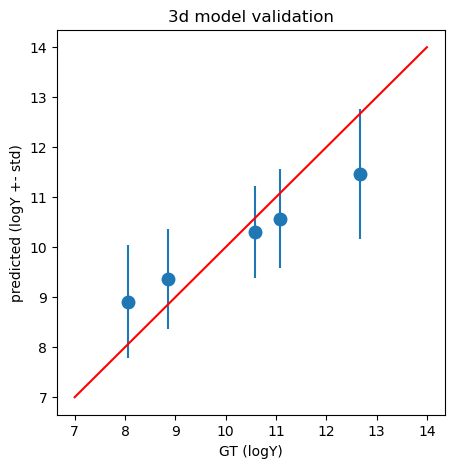
\includegraphics[width=.6\textwidth]{latex_template/figs/val.png}
\caption{\textbf{Validation using posterior predictive check. } The validation was done on the 3D GP model without the hydrologic region as the inputs. The x-axis is the ground-truth (GT) output, the y-axis is the predicted value from HMC with error bars showing the variance from sampling. Both axes are shown on log scales. }
\label{fig:val}
\end{figure*}



For the model implementation, we used the HMC sampling results implemented by Stan for our analysis results. The learned coefficients $\beta$ are plotted on Figure \ref{fig:coeff} top, ordered based on the value. The coefficient for the prescribed fire is shown on black. We see that depends on the hydrologic region the wildfire impact largely vary, with San Francsisco Bay area having least severity and the Central coast having a largest severity. We also realized that the prescribed fire, while having the negative coefficients based on the sampling average, has relatively small impact on the wildfire severity. 

We also fit the same model using the same data and the same model with the point estimation, which was done from \texttt{optimize} function in Cmdstan. This method uses L-BFGS algorithm to calculate the Maximum Likelihood estimate. By comparing the 11 coefficients learned (Figure \ref{fig:coeff} bottom), we found that there is a large discrepancy on the parameters estimated from MLE and HMC. This was also the case in the other parameters within the kernel functions. We suspect that MLE was finding the local optimam, therefore used the results from HMC in the following steps. An alternative reason is the parameter identifiability but we will not explore this potential cause here. 




\begin{figure*}[!t]
  \centering
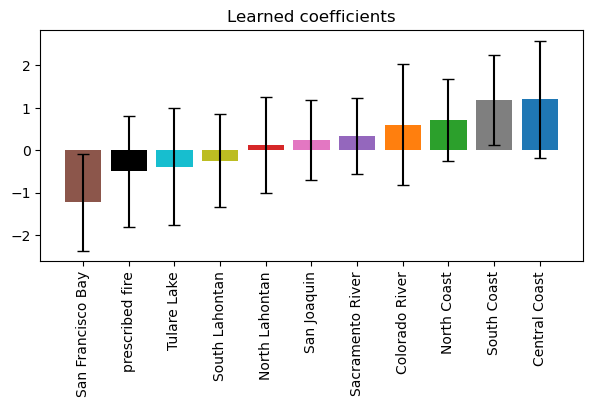
\includegraphics[width=0.9\textwidth]{latex_template/figs/betas.png}
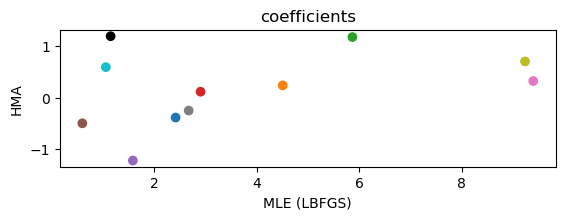
\includegraphics[width=0.9\textwidth]{latex_template/figs/hmc_mle.png}
\caption{\textbf{Parameter estimation results.} Top plot is the estimated mean of the coefficients ($\beta$ ) for all 11 explanatory variables listed. The error bars represent the standard deviation of MCMC samplings. The bottom panel is the comparison of estimated coefficients between MLE using Stan's \texttt{optimization} algorithm (x-axis) versus those estimated using MCMC (y-axis). The colors corerespond to the top panel. }
\label{fig:coeff}
\end{figure*}






Lastly, we overlapped the predicted output (burned area by wildfire occurrences) with the original map of California, as well as the prescribed burn locations. Consistent with the validation results in Figure \ref{fig:val}, the output of the burned area from the model have much less variance than the burned area in the training data. This is possibly caused by the lack of training data - only the locations where prescribed burn data is available was used for the testing, but this was not the case for training. In the other words, in the training data, many of the prescribed burn area was zero whereas in the testing this input was always larger than zero. Therefore, considered the lack of the data, this result was not surprising. Also we found that the predicted fires are larger in the coastal area (North, Central and South coast) than the inshore (inner land) or mountain area in general, which is counter-intuitive. This is possibly caused by lacking the training data in the coastal area. 




\begin{figure*}[!t]
  \centering
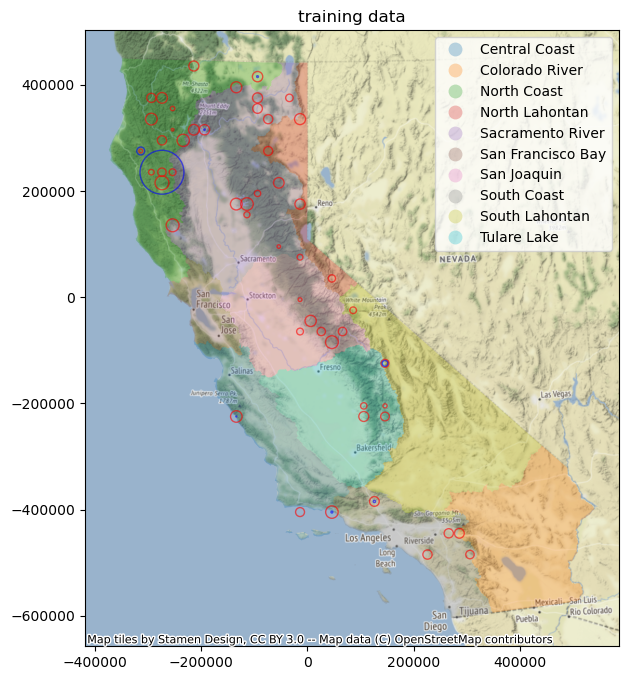
\includegraphics[width=0.49\textwidth]{latex_template/figs/trained_rez.png}
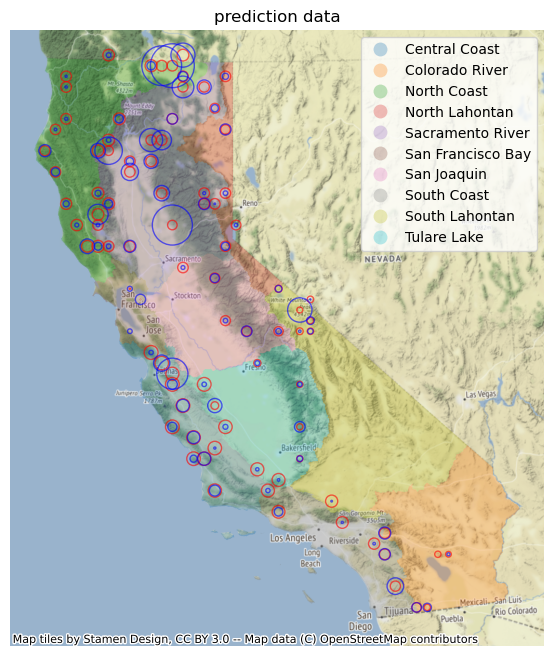
\includegraphics[width=0.49\textwidth]{latex_template/figs/predicted_rez.png}
\caption{\textbf{Relationships between the burned area from wildfire (red circles) and the prescribed fire (blue circles). } Left panel shows the explanatory variables (hydrologic regions and prescribed burn locations) overlaid with the wildfire burned area and the geographical locations in California. Right panel shows all the explanatory variables overlaid with the the geographical locations in California, as well as \textit{predicted} wildfire burned area. Prescribed fire are shown in blue circles and ground-truth or predicted burned area are shown in red circles. The size of the circles  corresponds to the burned area.}
\label{fig:pred}
\end{figure*}





\section{Discussion}
2D Gaussian Process in the field of geostatistical is essentially the ``kringing'' problem, but cannot incorporate the other covariates effectively. Using the flexibility of the sampling approach in Stan, we extended the simple 2D GP by incorporating the explanatory variables, which gives more flexibility in modeling and allows us to be more expressive on what factors should be considered. Using this model we concluded that some hydrologic region has a large impact on the wildfire severity than the prescribed burns. 


The discrepancy on the point estimation and the HMC estimation we see from this analysis might be caused by the suboptimal model specification, which can lead to poor parameter identifiability. This needs to be further investigated. It is possible that point estimation found the local minima whereas the sampling approach found the global optimum. 

Many covariates are not included due to the limited data and resource for the scope of this analysis. Some of the relevant factors that were not included in the analysis are topographical data that captures the landscapes more accurately, as well as the vegetation conditions. More importantly, in order to assess the relationships between these factors, the time of occurrences are very important, especially for the prescribed burn and the wildfire occurrences. The aimi of this report is to provide the resource and hte modeling framework therefore in the future with this framwork we hope these unaddressed points can be resolved eventually. 


\clearpage
\bibliographystyle{unsrt}
\bibliography{ref}















\clearpage
\section{Appendix}
\makeatother
% \paragraph*{\textnormal{S1 Appendix}.}
This is Stan code. Note that a large part of this was adopted from \cite{riutort2020practical}. 

\begin{verbatim}
// exact GP
functions {
	#GP 2D (analytical predicting)  # only use one alpha 
	vector gp12_pred_rng(real[] x1_grid, real[] x2_grid,
					 vector y1, real[] x1, real[] x2,
					 real alpha, real rho1, real rho2, real sigma, real delta) {
		int Nsample = rows(y1);
		int N2 = size(x1_grid);
		vector[N2] mu;
		{
		  matrix[Nsample, Nsample] K =   cov_exp_quad(x1, alpha, rho1).*cov_exp_quad(x2, 1, rho2)  ## N x N
+ diag_matrix(rep_vector(square(sigma), Nsample));
		  matrix[Nsample, Nsample] L_K = cholesky_decompose(K);
		  vector[Nsample] L_K_div_y1 = mdivide_left_tri_low(L_K, y1);
		  vector[Nsample] K_div_y1 = mdivide_right_tri_low(L_K_div_y1', L_K)';
		  matrix[Nsample, N2] k_x1_x2 = cov_exp_quad(x1, x1_grid, alpha, rho1).*cov_exp_quad(x2, x2_grid, 1, rho2);  ## N x N*
		  vector[N2] f2_mu = (k_x1_x2' * K_div_y1); //'
		  matrix[Nsample, N2] v_pred = mdivide_left_tri_low(L_K, k_x1_x2);
		  matrix[N2, N2] cov_f2 = cov_exp_quad(x1_grid, alpha, rho1).*cov_exp_quad(x2_grid, 1, rho2) - v_pred' * v_pred
								  + diag_matrix(rep_vector(delta, N2)); //'  N* x N*
		  mu = multi_normal_rng(f2_mu, cov_f2);
		}
		return mu;
	}
	
	#Kernel 2D
	matrix ker_gp12(real[] x1, real[] x2, real sdgp, real lscale1, real lscale2, real sigma) { 
		matrix[size(x1), size(x1)] cov;
		cov = cov_exp_quad(x1, sdgp, lscale1).*cov_exp_quad(x2, 1, lscale2);
		for (n in 1:size(x1)) {
			cov[n, n] = cov[n, n] + square(sigma);
		}
		return cholesky_decompose(cov);
	}
}

data {
	int<lower=1> Nsample;
	int Npred;
	int<lower=1> D;
	vector[2] x[Nsample];
    vector[D] z[Nsample];
	vector[Nsample] log_y;
	vector[2] x_grid[Npred];
    vector[D] z_grid[Npred];
}

transformed data{
	vector[Nsample] zeros = rep_vector(0, Nsample);
    vector[Nsample] y = exp(log_y);
    # real logymean = mean(log_y);
    # real logysd = sd(log_y);
    # vector[Nsample] log_yn = (log_y - logymean)/logysd;
}

parameters {
	real<lower=0> rho[2];
    row_vector[D] beta;
	real<lower=0> sigma;
    real<lower=0> eta;
	real<lower=0> alpha[2];
    vector[Nsample] f;
}

transformed parameters{
	vector[Nsample] g;
    vector[Npred] g_grid;
    matrix[Nsample,Nsample] L_K;
	L_K = ker_gp12(x[,1], x[,2], alpha[1], rho[1], rho[2], sigma);
    for (i in 1:Nsample){
      g[i] = beta*z[i];
    }
    for (i in 1:Npred){
      g_grid[i] = beta*z_grid[i];
    }
}

model{
	rho ~ inv_gamma(1,1);
	sigma ~ normal(0,1);
    eta ~ normal(0,1);
	alpha ~ normal(0,2);
    beta ~ normal(0,2);    
    f ~ multi_normal_cholesky(zeros, L_K);
    log_y ~ normal(f + g, eta);
}

generated quantities{
	vector[Npred] f_grid;
	vector[Npred] y_grid_predict;
	vector[Npred] log_y_grid_predict;
    real pred_log_y;

	#GP 2D (Analytical prediction)
	f_grid = gp12_pred_rng(x_grid[,1], x_grid[,2], log_y - g, x[,1], x[,2], alpha[1], rho[1], rho[2], sigma, 1e-10);
    
	for (i in 1:Npred){
		log_y_grid_predict[i] = normal_rng(f_grid[i] + g_grid[i], sigma); 
        y_grid_predict[i] = exp(log_y_grid_predict[i]);
	}
}
\end{verbatim}


\end{document}
